\chapter{Ergebnis}
\section{Sensormessungen mit dem siot.net Sensorcenter}
Um das Ergebnis beider entwickelten Programmartefakte zu testen, wurden einige Messungen mit dem siot.net Sensorcenter getätigt, welcher die siot.net Gateway Library integriert. Als Messinstrument wurde der Herzfrequenzmesser der Motorola Moto 360 Smartwatch verwendet. Für die Herzfrequenzmessungen sind drei verschiedene Testpersonen gewählt worden. Für erste Tests wurden die Daten, auf der Abbildung 11.1 visualisierte Node-RED Instanz, manuell ausgewertet. Sobald das siot.io Dashboard verfügbar war, wurden alle Test nochmals Durchgeführt, um die Messwerte dort zu analysiert.
\begin{figure}[H]
  \centering
  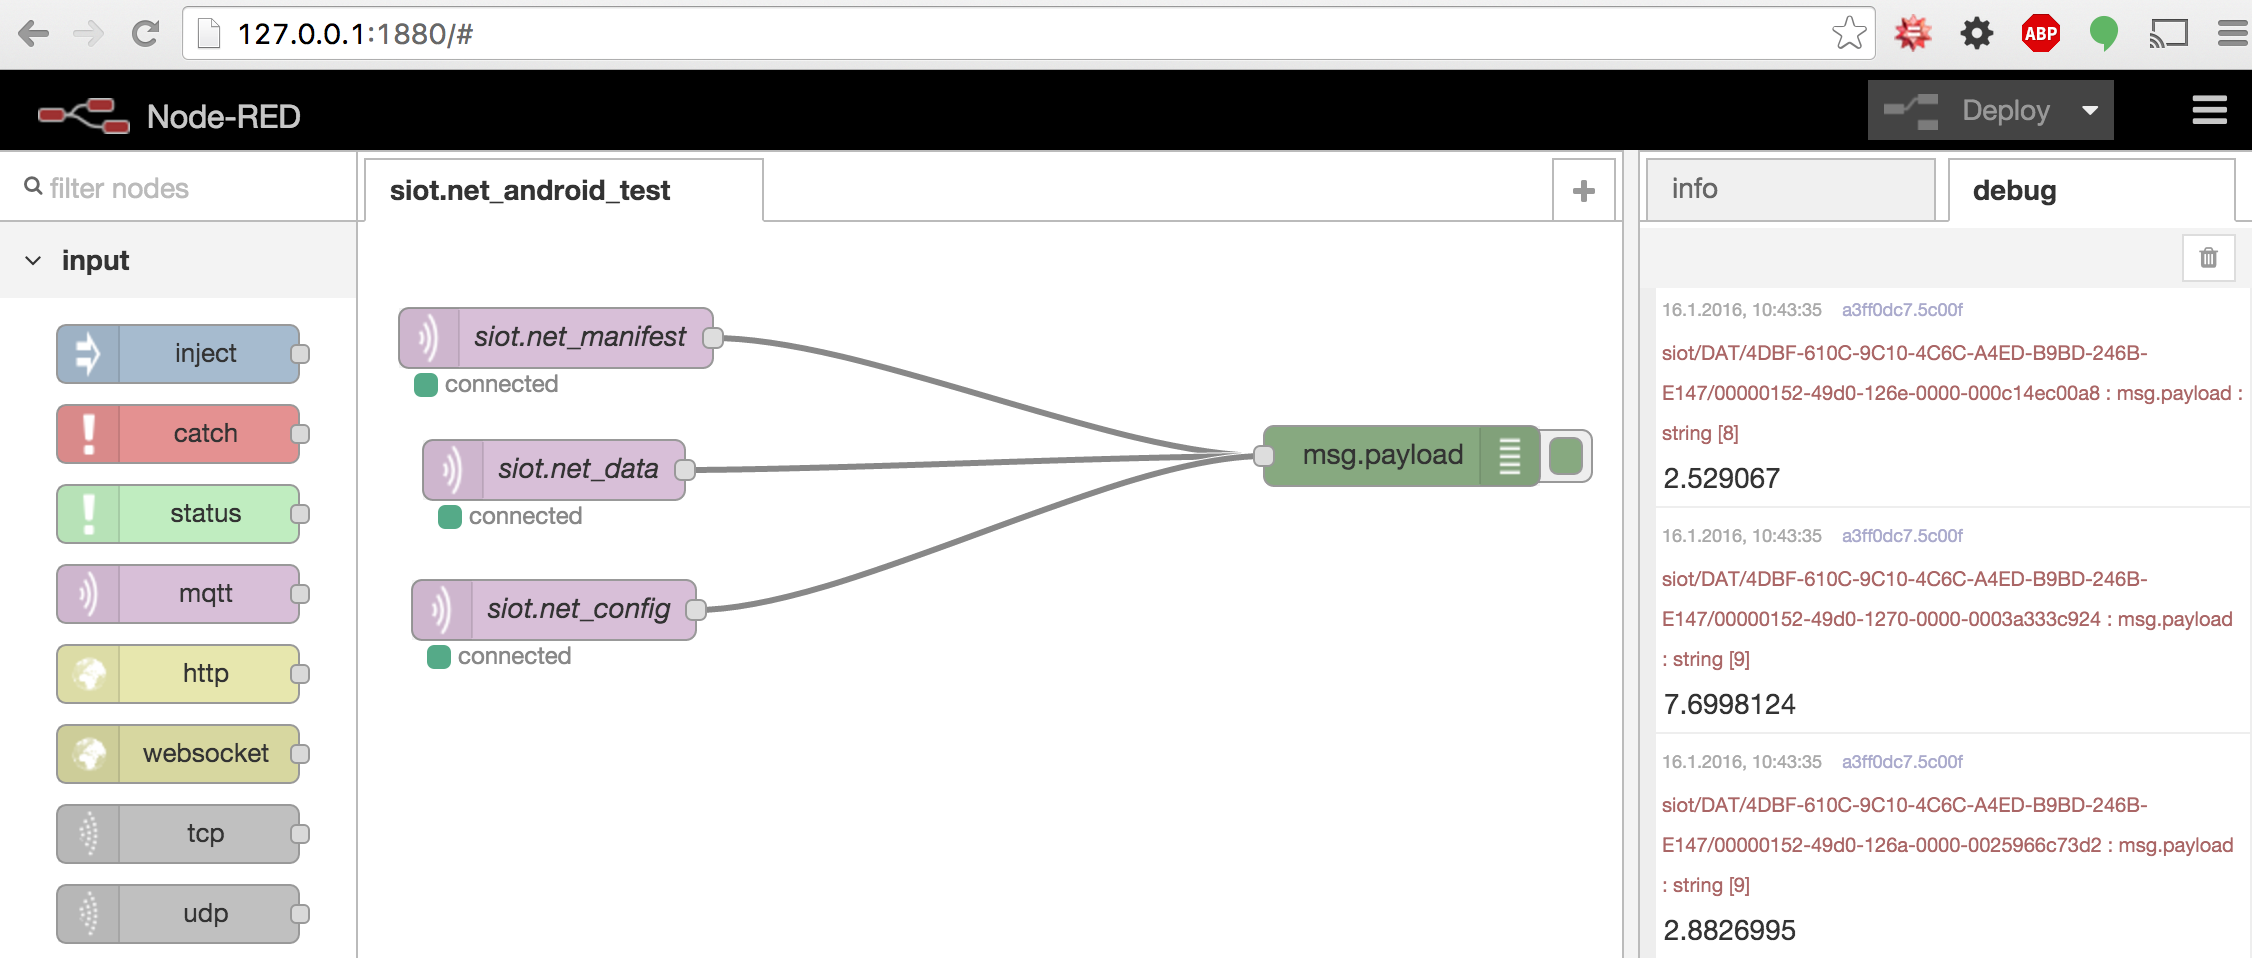
\includegraphics[scale=0.4]{98_Bilder/11_Ergebnis/nodeRED}
  \caption[Node-RED Testflow]{Verwendete Node-RED Fluss zum Testdaten empfangen}
\end{figure}
\subsection{Voraussetzungen}
Es wurden drei Testpersonen gewählt, zwei männliche und eine weibliche. Eine männliche und die weibliche Person sind im frühen Erwachsenenalter (18-35), die zweite männliche Person ist im mittleren Alter (35-65), diese Person weist eine Arrhythmie auf. Die Messungen wurden jeweils sitzend ohne körperliche Anstrengung durchgeführt.
\subsection{Testresultate}
Bei der ersten und zweiten Testperson sind die Messwerte kontinuierlich gemessen und übermittelt worden. Dies ist auf der Node-RED Instanz und auf dem siot.io Dashboard Graphen ersichtlich. Genau so ist zu erkennen, dass bei der dritten Person kein Puls gemessen werden konnte.
\subsubsection{Testperson 1}
\begin{figure}[H]
  \centering
  \includegraphics[scale=0.375]{98_Bilder/11_Ergebnis/heartrateSPnodeRED}
  \caption[Node-RED Messwerte Person 1]{Messwerte der ersten Testperson, ersichtlich in Node-RED}
\end{figure}
\begin{figure}[H]
  \centering
  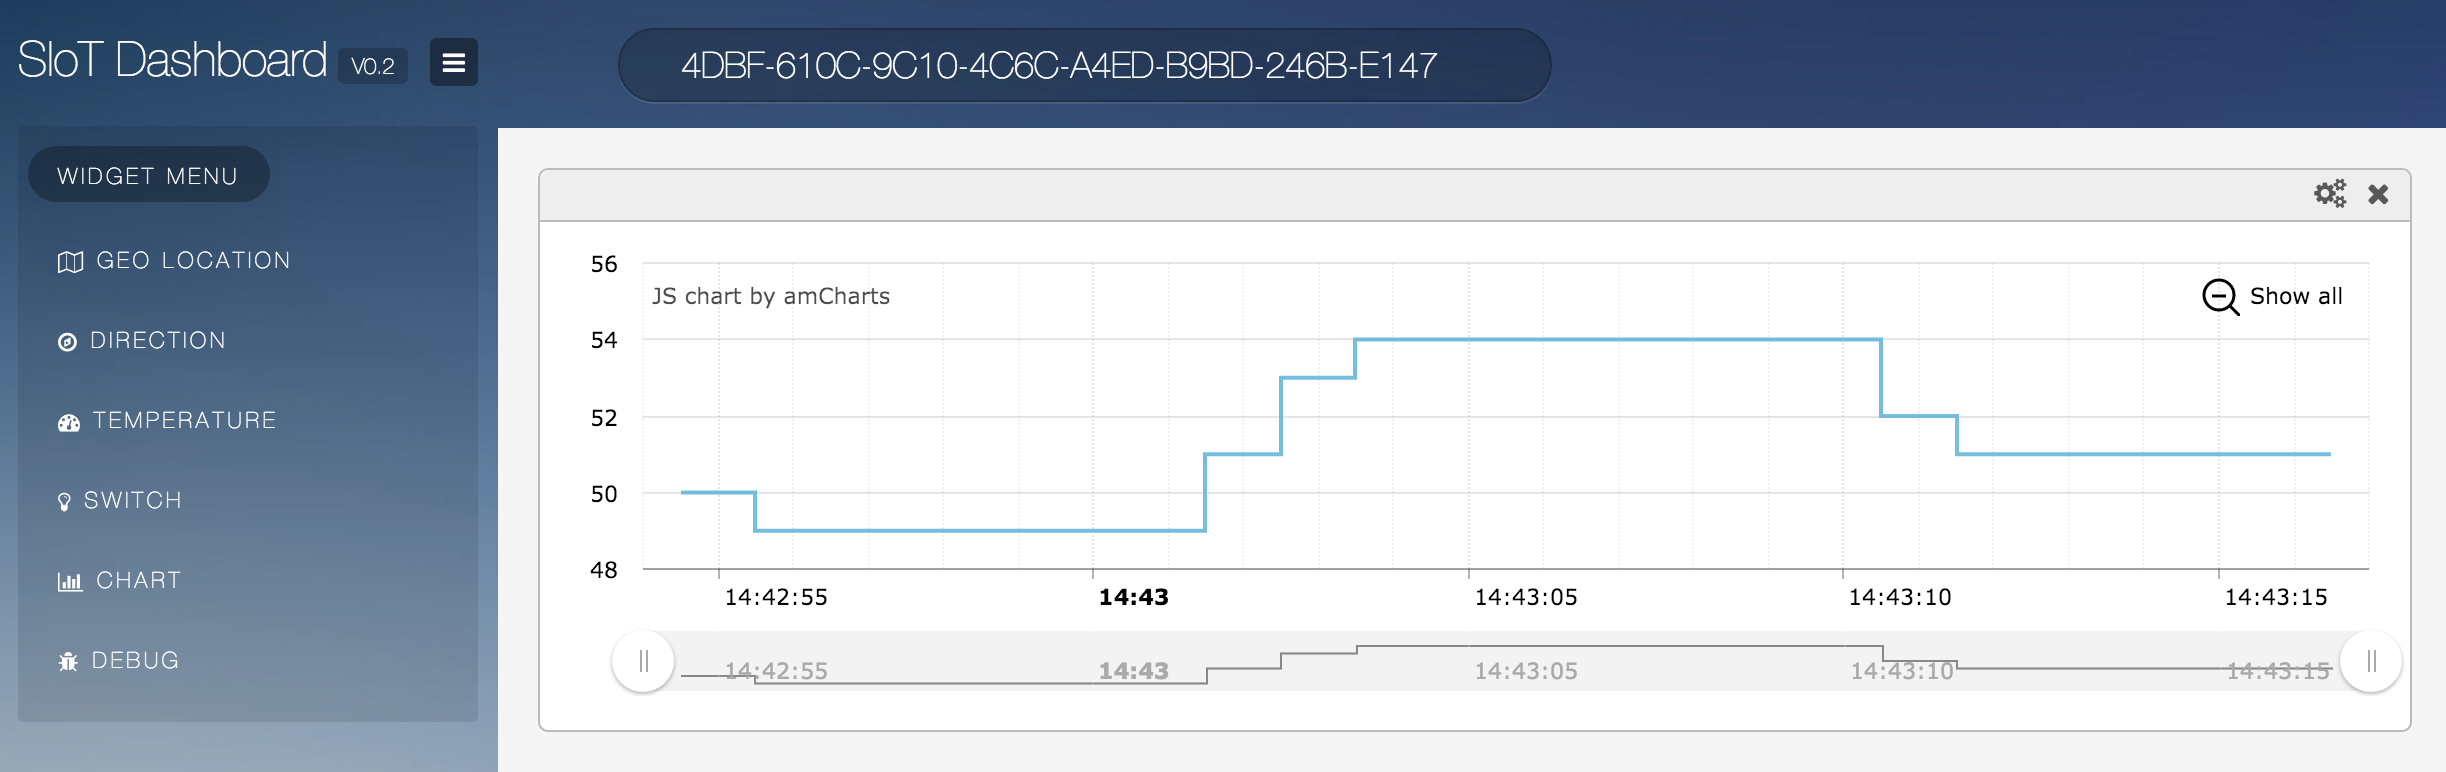
\includegraphics[scale=0.375]{98_Bilder/11_Ergebnis/heartrateSPsiotio}
  \caption[siot.io Dashboard Graph Person 1]{Der Herzfrequenzgraph auf siot.io der Testperson 1}
\end{figure}
\subsubsection{Testperson 2}
\begin{figure}[H]
  \centering
  \includegraphics[scale=0.375]{98_Bilder/11_Ergebnis/heartrateCRnodeRED}
  \caption[Node-RED Messwerte Person 2]{Messwerte der zweiten Testperson, ersichtlich in Node-RED}
\end{figure}
\begin{figure}[H]
  \centering
  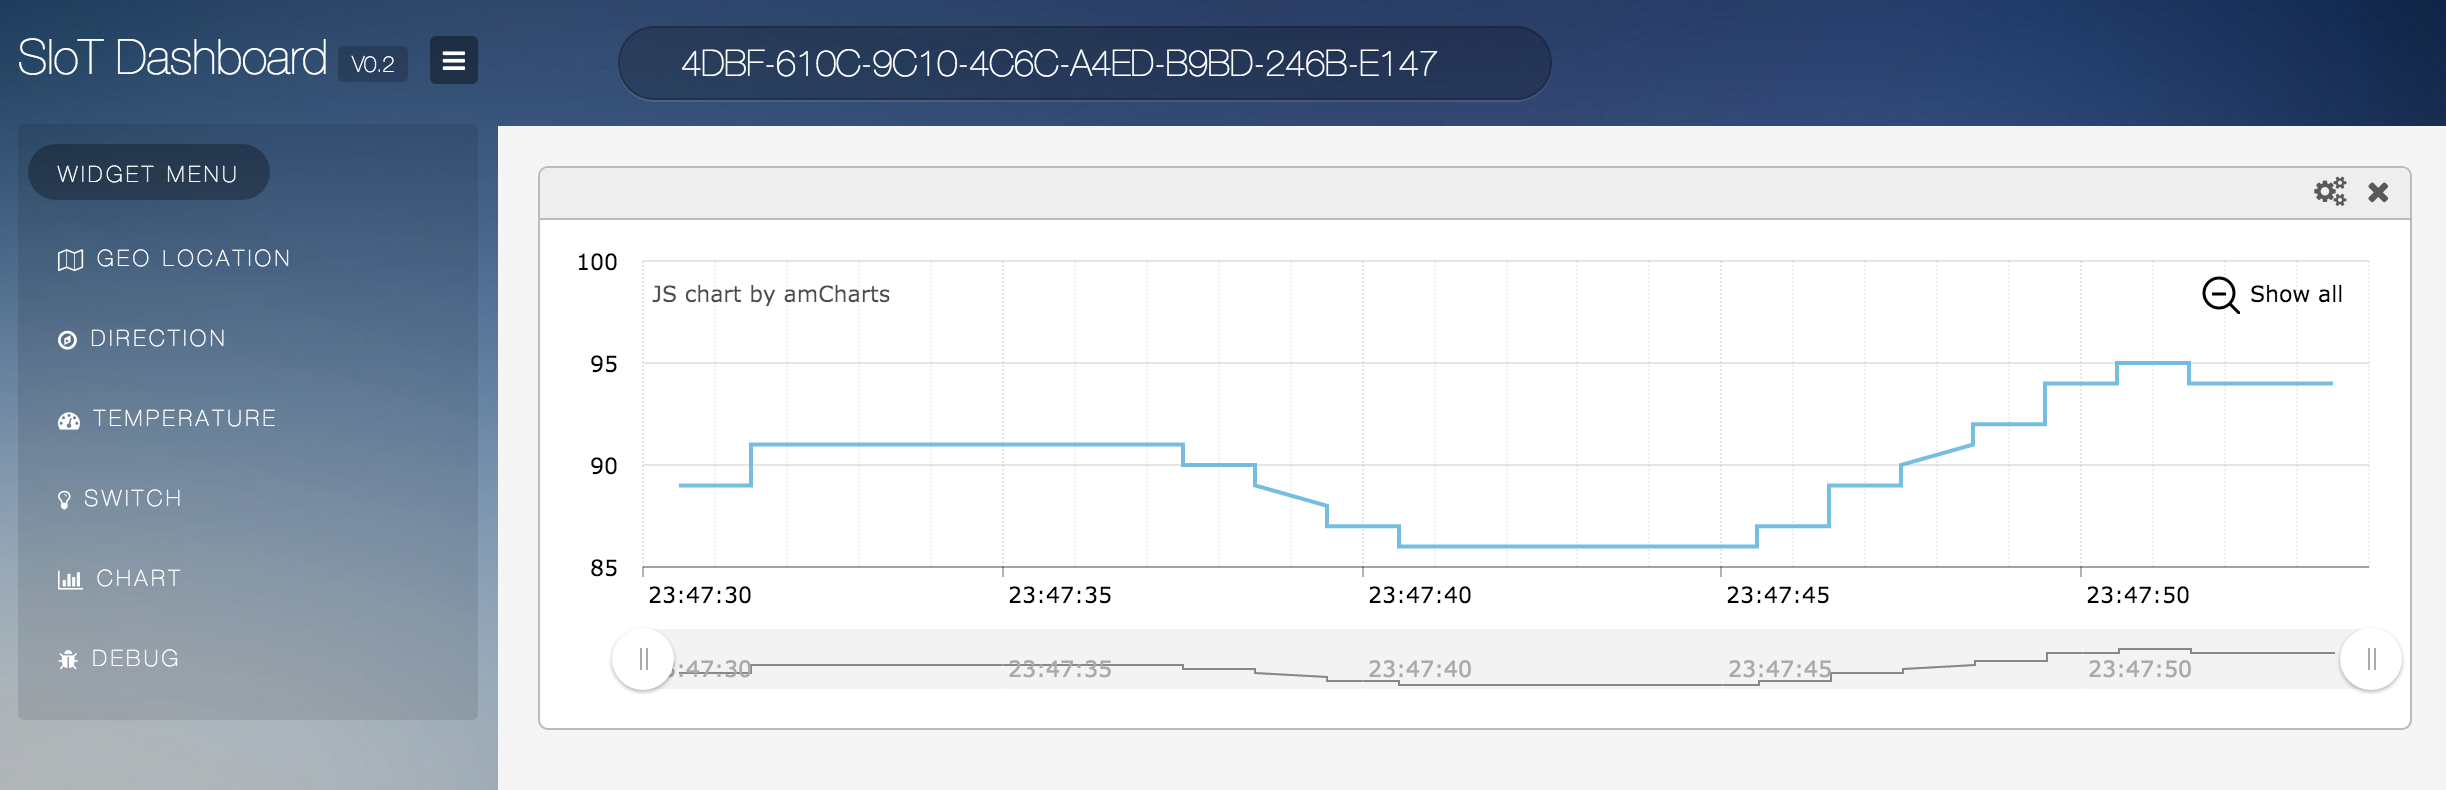
\includegraphics[scale=0.375]{98_Bilder/11_Ergebnis/heartrateCRsiotio}
  \caption[siot.io Dashboard Graph Person 2]{Der Herzfrequenzgraph auf siot.io der Testperson 2}
\end{figure}
\subsubsection{Testperson 3}
\begin{figure}[H]
  \centering
  \includegraphics[scale=0.375]{98_Bilder/11_Ergebnis/heartrateADnodeRED}
  \caption[Node-RED Messwerte Person 3]{Messwerte der dritten Testperson, ersichtlich in Node-RED}
\end{figure}
\begin{figure}[H]
  \centering
  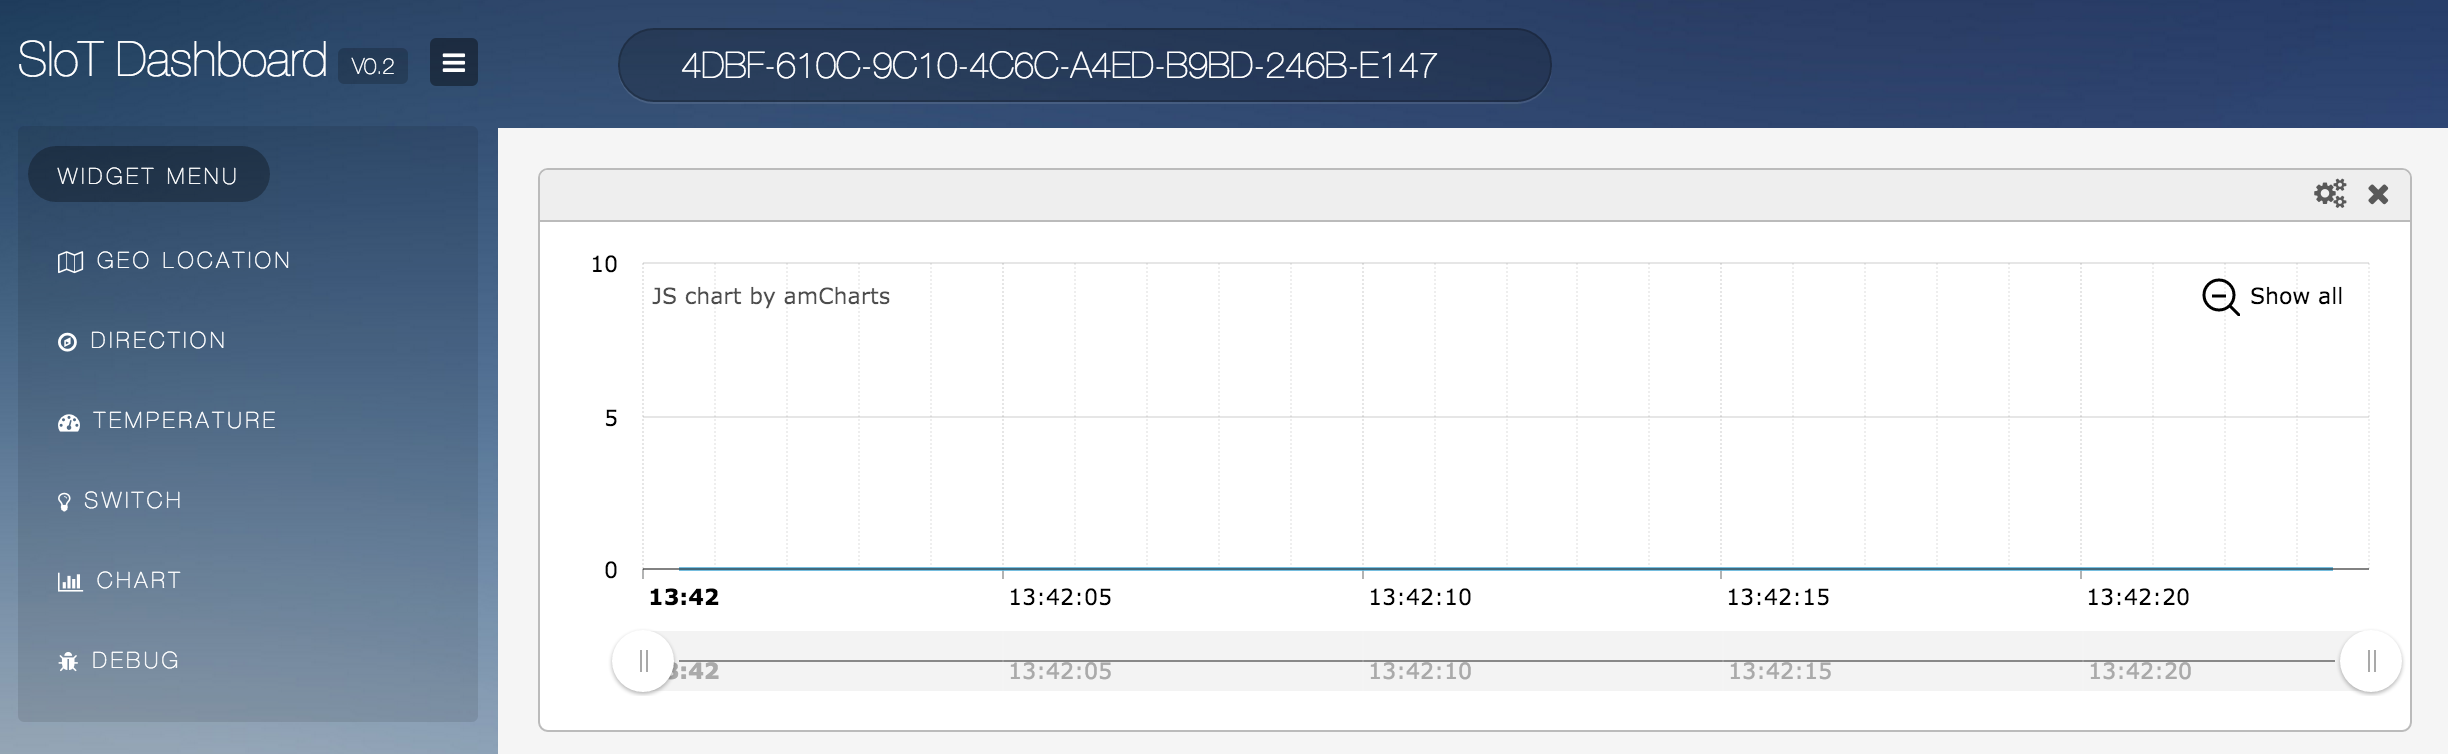
\includegraphics[scale=0.375]{98_Bilder/11_Ergebnis/heartrateADsiotio}
  \caption[siot.io Dashboard Graph Person 3]{Der Herzfrequenzgraph auf siot.io der Testperson 3}
\end{figure}
\section{Beurteilung}
Die Tests wurden mehrmals durchgeführt, ausser bei der dritten Testperson. Das Ergebnis bestätigte, dass die Werte immer im ähnlichen Bereich befanden. Jedoch ist sie nicht immer zuverlässig. Es konnte beobachtet werden, dass wenn der Arm stark bewegt wurde, der Herzfrequenzmesser den Puls nicht mehr korrekt berechnen konnte. In diesen Fällen versendet die Smartwatch eine lange Periode den zuletzt gemessenen Wert. Nach der Rekalibrierung, was meist (in über 60\% der Fälle) automatisch geschieht, wurden wieder korrekte Messwerte empfangen.\\
Die korrekt gemessenen Werte, weisen eine kleine Abweichung zu einem Brustgurt auf. Der Differenzwert betrug durchschnittlich -4.5 Herzschläge. Dies wurde in einem Selbsttest, mit einem Brustgurt der Marke Kettler und einem Sportgerät desselben Herstellers, verifiziert. Bei Personen (z.B Testperson 3), welche an einer Herzrhythmusstörung leiden, konnte gar keinen Puls ermittelt werden. Aus diesem Grund wurde dieser Test beim dritten Kandidaten abgebrochen.\\
Der Herzfrequenzmesser berechnet die Puls Rate aus einer Summe von Messungen in einem bestimmten Intervall. Bei der Unregelmässigkeit des Pulses konnte die Smartwatch keine zuverlässigen Werte messen, was zu einem Ausfall führte. Damit kann gesagt werden, dass der Pulsmesser bei Personen mit rhythmischer Herzfunktion zufriedenstellende Messwerte liefert. Jedoch bei Personen mit Arrhythmie kann dieser keine Messungen durchführen.
